\chapter{Implementation}
\label{sec:implementation}
\section{Communication classes}
We developed FastFlow's communication classes by extending the \ttt{ff\_node\_t} class, in such a way the developed classes can be used in any context where a \ttt{ff\_node\_t} can be used. However, we show that they naturally sit at the extremes of a pipeline building block, since they offer functionalities to receive and forward data from and through the network.\newline

The classes we implemented are strictly tied to the concepts of receiver and sender node, and they make use of Margo's capabilities of developing multi-endpoint services without requiring to manually handling progress loops. At the current stage of development, there is no personalized behaviour based on the endpoint which received a call to the registered RPCs. This represents the next main step in the evolution of the implemented classes. (De)Multiplexing, however, should be fairly easy to handle thanks to the internal mechanisms that Margo offers in order to identify the origin node which issued a request. Having personalized behaviour, depending on the specific endpoint, is very important to deal with the grouping concept introduced since the distributed version of FastFlow has been developed. Particularly pathological cases, where a personalized behaviour must be implemented given the specific endpoint on which the request is received, benefit from the automatized mechanisms offered by Margo. Moreover, the simplicity in handling multiple endpoints via the implemented classes allow to test a multitude of situations with little to no code changes.\newline

\subsection{Receiver node}
Receiver node is a FastFlow \texttt{ff\_node\_t} that relies on a Margo instance initialized with \texttt{MARGO\_SERVER\_MODE}. This allows the receiver node to wait for incoming RPC requests at the specified addresses. A list of addresses can be provided at initialization, translating in a receiver node listening for the same set of RPC functionalities on all of the provided endpoints. \hr{receiver-skeleton}{Listing} shows pseudo-code of the implemented receiver node.
\begin{lstlisting}[language=C++, style=mystyle, caption={Receiver node pseudo-code.}, label={receiver-skeleton}]{receiver-skeleton}
struct receiverStage: ff_node_t<Task> {
    std::vector<margo_instance_id> mids // Margo instances to be used during servicing

    // Parametrized constructor which registers all specified endpoints with the
    // provided configuration strings.
    receiverStage(std::array<char*> endpoints, std::array<char*> configs) {
        ...
        for(i < num_endpoints) {
            // init_endpoint initializes a Margo server instance on the provided address
            // and config string. The endpoint allocates a specific ES and pool to handle
            // all the requests coming through the specified address.
            // Returns an handle to the created Margo instance
            mids[i] = init_endpoint(endpoints[i], configs[i]);
            
            // Code to get the end address (to be forwarded and used by the sender node)
            // and various debugging can be put here, by using the mids generate by the init
            // phase
            ...
            
            // Use the initialized mids to register the set of RPCs that will be offered by
            // this receiver node.
            // Responses for the registered RPCs are disabled.
            register_service(mids[i])
        }
    
    }
    
    // The receiver node has nothing to do in the service method, it can simply wait
    // for termination of all the listening endpoints and forward the EOS at the end.
    // `task' parameter is ignored in this stage, since it acts as a sort of `endo-stream'
    // generator for the other stages in the pipe.
    Task* svc(Task* task) {
        wait_for_finalize(mids);
        return EOS;
    }
}
\end{lstlisting}

\subsection{Sender node}
Sender node, on the other hand, relies over Margo instance initialized with \texttt{MARGO\_CLIENT\_MODE}, since we do not expect this node to be listening on any RPC request for now.  The current version of the sender node allows to contact only a single endpoint at a given address. The address to contact for this specific node must be provided at initialization, and at the moment it is not possible to change the remote service address. In the next versions the possibility to contact multiple addresses, in order to implement the pathological grouping case described before, will be implemented following the same approach used for the receiver stage. Pseudo-code for this class is provided in \hr{sender-skeleton}{Listing}.

\begin{lstlisting}[language=C++, style=mystyle, caption={Sender node pseudo-code.}, label={sender-skeleton}]{sender-skeleton}
struct senderStage: ff_node_t<Task> {
    margo_instance_id       mid;        // Margo object to use for communications
    hg_addr_t               svr_addr;   // Server address listening for incoming RPCs

    senderStage(char* addr) {
        // Initialize the Margo instance as a client node and creates the necessary
        // objects to register RPC calls and addresses to issue the requests to the
        // specified address.
        mid = init_endpoint(addr);
        
        // This is the exact same function that is called by the receiver, but in this
        // case we don't need to provide implementation of the actual RPC function.
        register_service(mid);
    }

    Task* svc(Task* task) {
        // The task received by the previous stage is packed into the RPC registered
        // type and forwarded to the sender via an RPC call. The current node can
        // proceed since no response is expected.
        ff_rpc_in in = pack_task(task);
        forward_task(mid, in);
        return GO_ON;
    }

    void svc_end() {
        // Upon termination forwards a shutdown RPC to the connected receiver node.
        // The sender has nothing to do more than cleaning Margo resources. 
        forward_shutdown(mid, shutdown_id);
        finalize(mid);
    }
};
\end{lstlisting}

\section{RPC based service}
The developed classes allow distributed groups to communicate through a fixed set of RPC calls, which are shared among receiver and sender nodes and used for all the communications between the various groups. Two RPCs are offered by the communication service, and they refer to:
\begin{itemize}
    \item \texttt{ff\_rpc}: this RPC is used during the whole lifetime of the FastFlow application, and it is used by the sender node, upon reception of a stream element, to forward the current stream element to the receiver node it is connected to. The sender node packs the data in the RPC input type, as described in \textbf{\S\ref{sec:rpc-reg}}, and ships them issuing a forward call to the connected endpoint. Since no response is expected from the RPC call, the sender can proceed immediately.
    \item \texttt{ff\_rpc\_shutdown}: this RPC is only used upon reception of an EOS object from the stream. In this case no data needs to be sent through the network, but only a signal that the stream has ended, in order to allow the receiving node to gracefully terminate its execution and forward EOS accordingly to the local group's nodes. Signaling an EOS propagates through the network, since the receiver node will generate an actual EOS object when the \texttt{ff\_rpc\_shutdown} callback is executed that will allow local nodes to terminate as per FastFlow's execution flow. At that point, the next sender node will issue an end-of-stream RPC and the whole FastFlow application will terminate. Note, however, that a receiver node will not forward an EOS object unless all the listening endpoints have received a shutdown RPC.
\end{itemize}

It is important to point out that this set of RPC callbacks need to be registered only once per Margo instance. This means that, once for each listening endpoint, the receiver node must register the same set of RPCs, but it is completely agnostic on the number of nodes that will issue RPC requests on the same endpoint. 

\section{Splitting taxonomy}
In this section we analyze the characteristics of different connections that take place between remotely connected groups, we show that very specific types can be determined whether the splitting happens in a \textit{horizontal} or \textit{vertical} fashion. We describe the specific categories depending on different splitting strategies. To better explain the identified categories, we introduce the concepts of \textit{level}, \textit{horizontal} and \textit{vertical} splits. Considering a generic FastFlow application as a pipeline of stages, we naturally associate a \textit{level} to each stage incrementally. In addition, we define as \textit{horizontal} a split which creates two groups sitting at the same level of the original pipeline, instead we define as \textit{vertical} a split which creates groups operating at two different levels of the pipeline. Note, however, that a \textit{vertical} split can internally contain further \textit{vertical} or \textit{horizontal} splits. Given these definitions, we can identify two categories that describe each of the connections in remotely-connected groups, specifically:
\begin{itemize}
    \item \textit{internal}: elements to be sent/received are related to a connection that takes place between groups that are split horizontally. Connections of this type can be linked to splittings that divides an original FastFlow building block in two groups belonging to the same pipeline level, for example an \textit{all-to-all} building block divided by distributing left and right workers in two groups;
    \item \textit{external}: elements to be sent/received are related to connections that take place between two groups at different levels of the original pipeline. These connections are typically related to vertical splits of the original FastFlow application.
\end{itemize}

To better illustrate this taxonomy, we present a simple example which contains every concept we introduced up to now. In \hr{fig:original-a2a}{Figure} there is a sample FastFlow application composed of an \textit{all-to-all} building block with two left workers and two right workers. By performing an \textit{horizontal} ``cut'', we want to split the \textit{all-to-all} in two different groups, each of them with one left worker and one right worker. If we consider this \textit{all-to-all} block to be in the middle of a pipeline, the groups will finally be as depicted in \hr{fig:taxonomy}{Figure}. We show the structure of the main software entities that handle the splitting. As we can see, the amount of nodes participating in the application increases to facilitate communication between remote groups, both via \textit{internal} connections (LS1 to RS2) and via \textit{external} ones (ff\_receiver to LS2).\newline

We will proceed now by describing the bigger picture by delving into particulars and explaining each of the involved parts and messy communication lines. The reasoning is very simple once the way communications are handled is clear, but it can seem pretty complicated at the start. We depicted in different colours the data flow which involve a stream element as the same ``origin'' object. When the colour of a communication line changes, also the provenance attached to the considered object will change. We describe in the following the different concepts depicted in the picture below:
\begin{itemize}
	\item left/right box: they are abstracted representations of \textit{internal} nodes in remotely connected groups. Left and right boxes of horizontally split groups, belonging to the same original building block, are logically connected by mean of their own local sender and receiver nodes. Since they respectively emulate a left and right worker, a stream element received by a left box (and hence originally shipped by a right box in a remote group) will be forwarded to a right worker in the current local group.
	\item red channel: carries stream elements which are part of the normal flow of execution, for example streaming elements flowing through the stage of a pipeline one after the other.
	\item purple/green channel: represents \textit{internal} connection channels.  They allow communication between boxes of different groups in order to maintain the \textit{all-to-all} semantic in a distributed environment.
\end{itemize}

The connections, internally, are determined by each remote group by means of the configuration file provided upon initialization and by the information that are exchanged during the startup phase. In this way, each receiver/sender node can associate correctly the ID of each channel to the various entities that are created after the splitting is performed.

\begin{figure}[H]
	\centering
	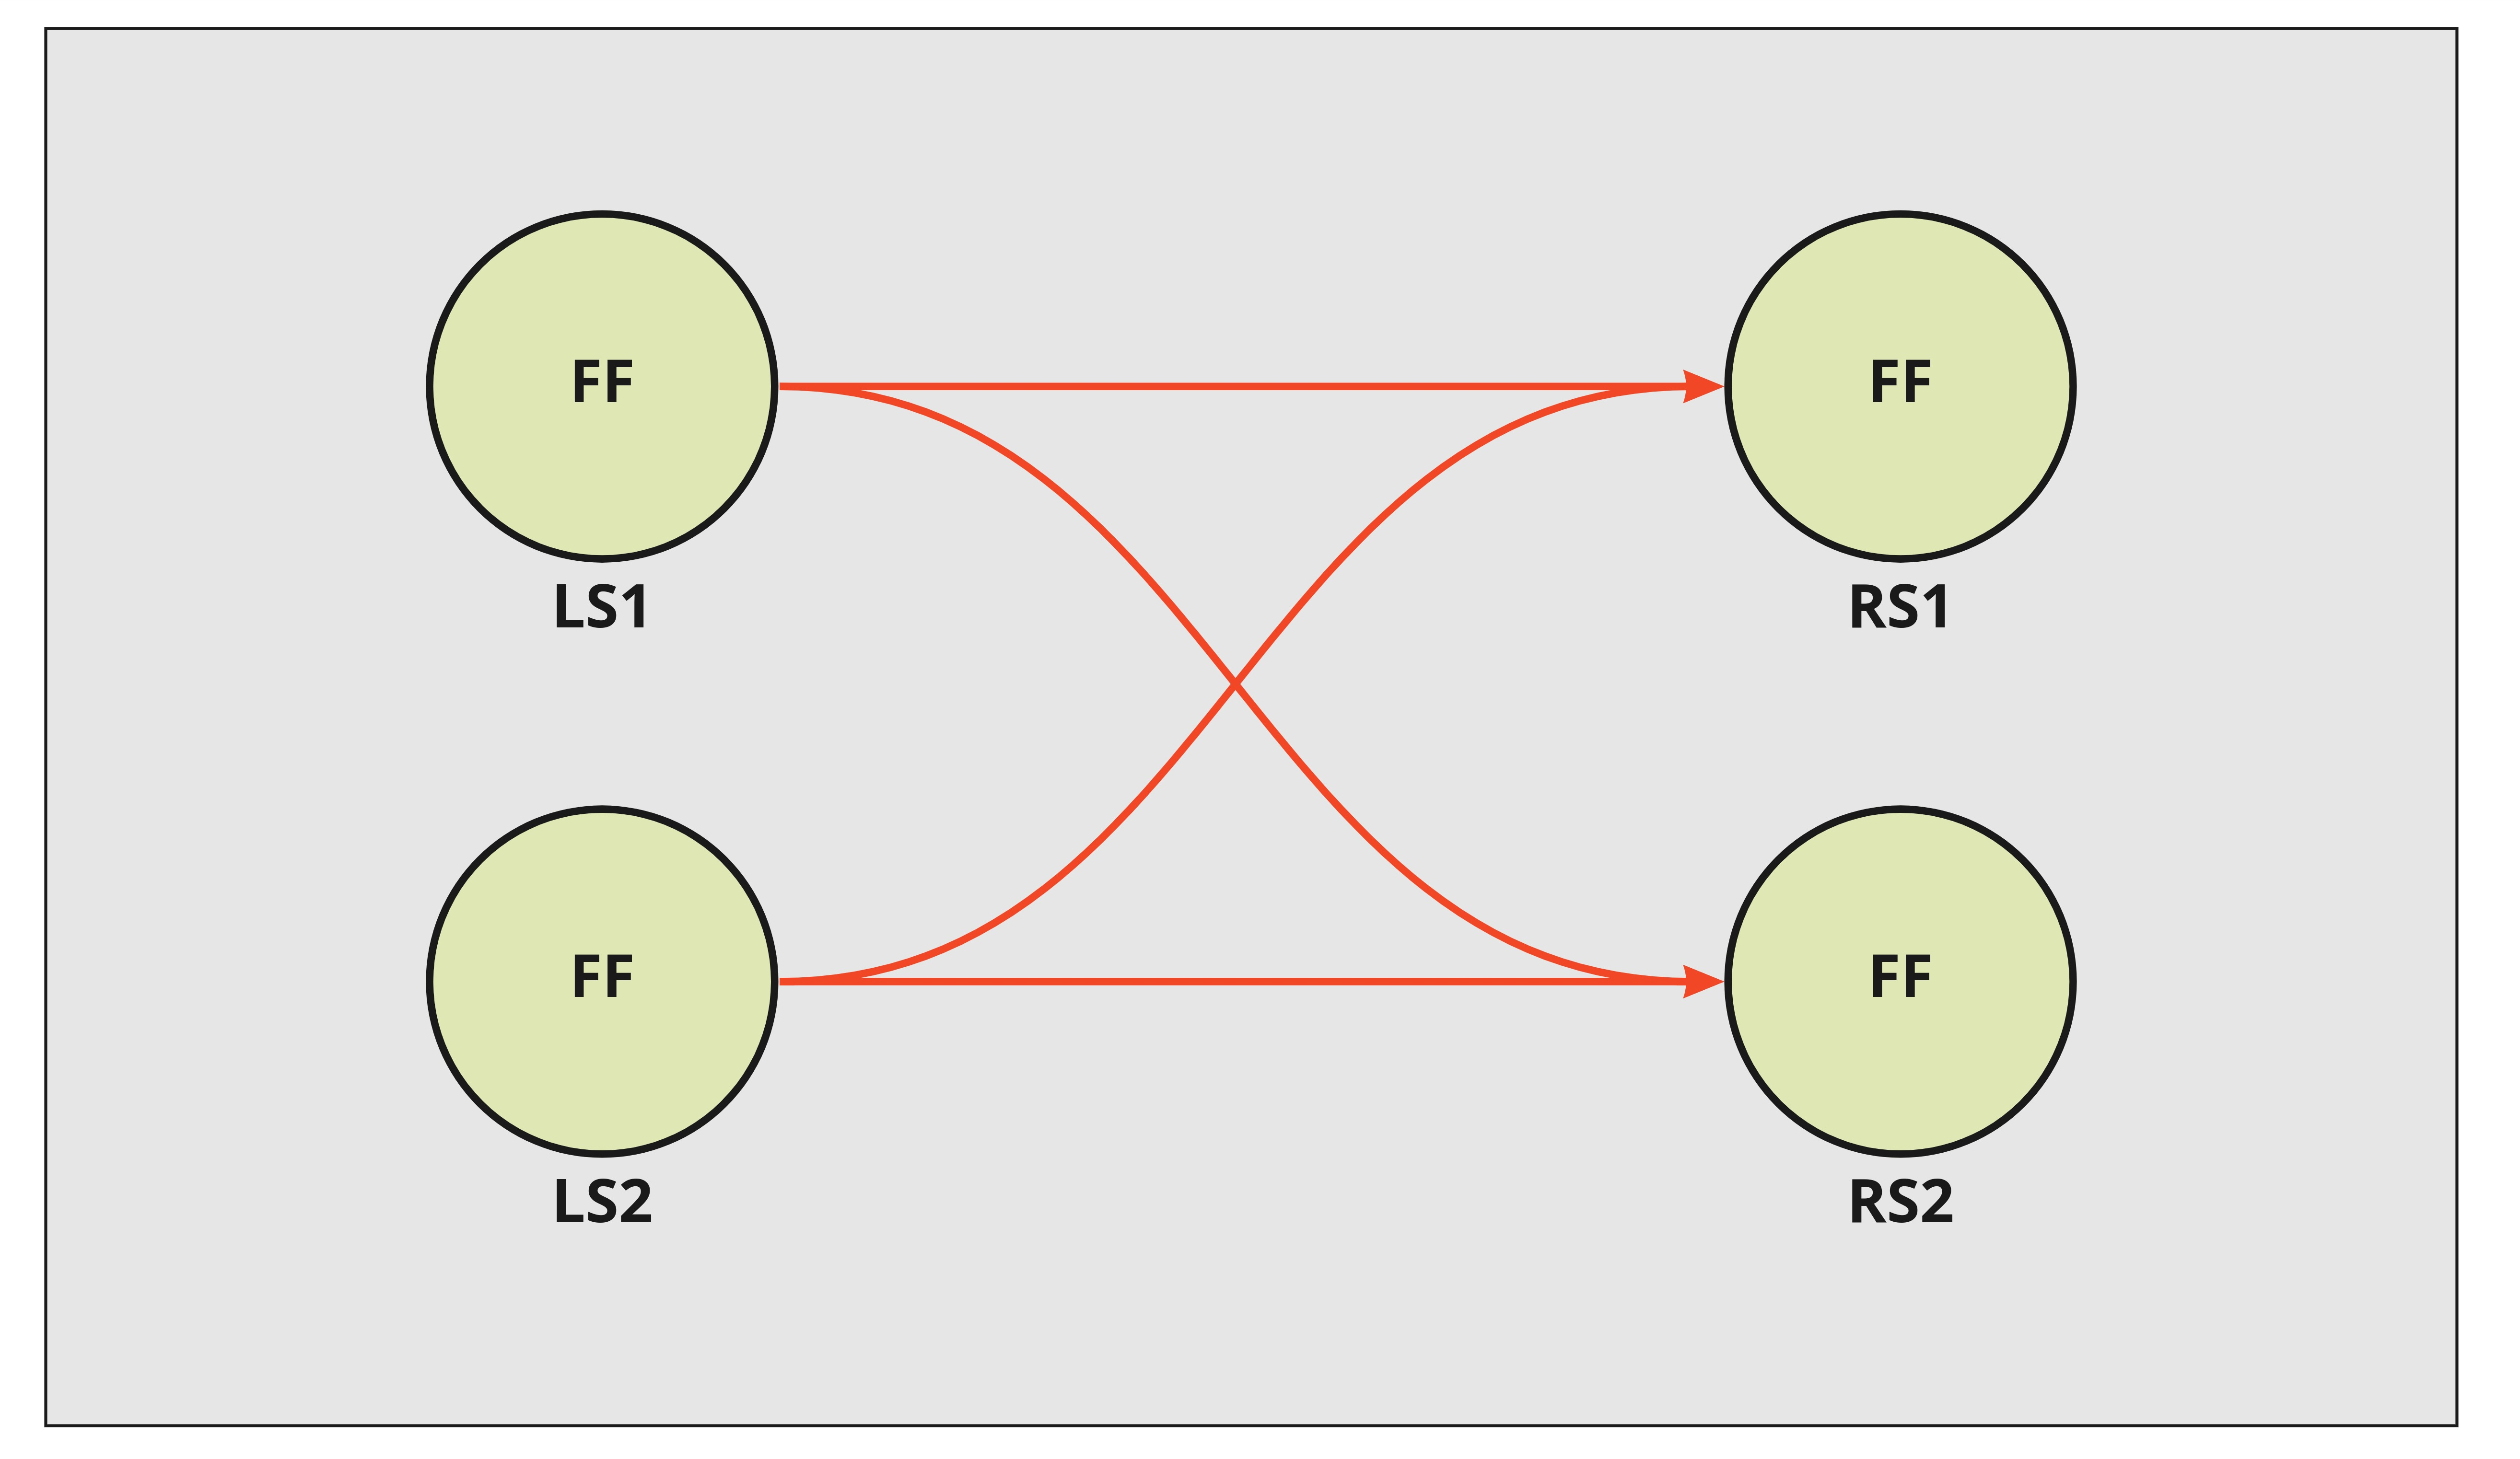
\includegraphics[width=0.5\linewidth]{res/original-a2a.jpg}
	\caption{Sample A2A building block.}
	\label{fig:original-a2a}
\end{figure}

\begin{figure}[H]
    \centering
    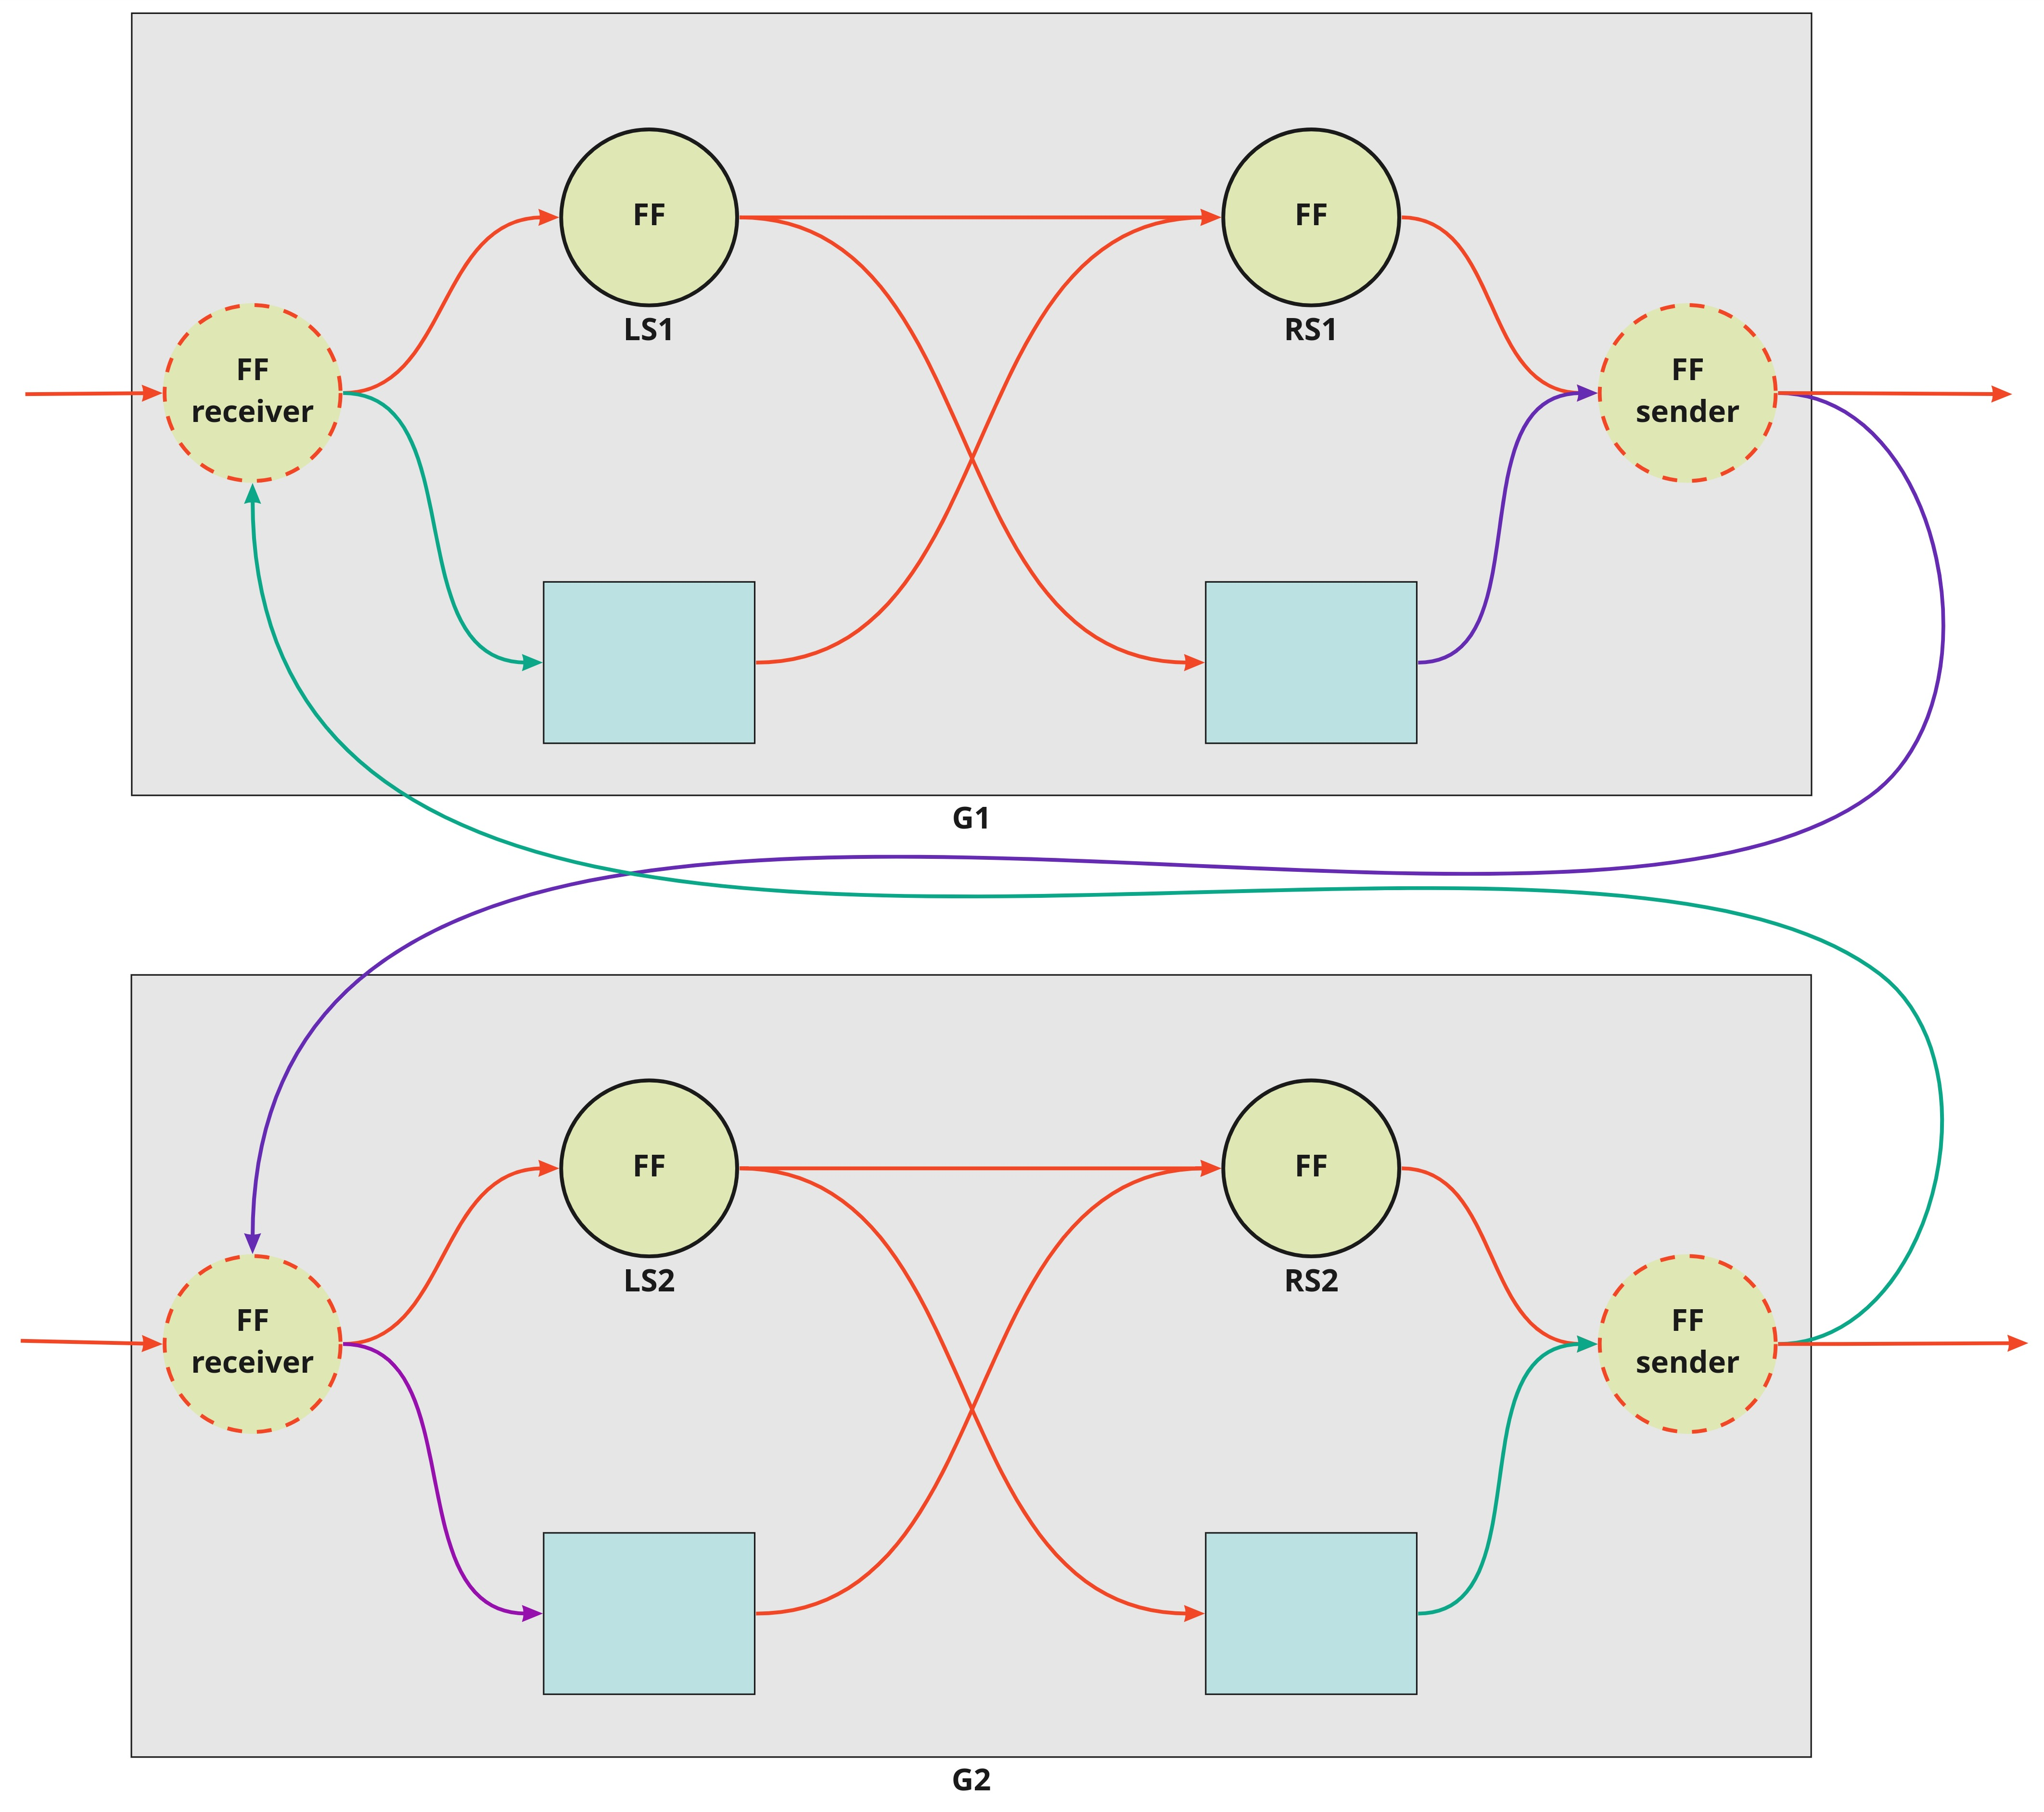
\includegraphics[width=0.8\linewidth]{res/taxonomy.jpg}
    \caption{Pathological case representing the splitting of an A2A node into two groups which needs to communicate internally in order to retain the original semantic of the A2A building block.}
    \label{fig:taxonomy}
\end{figure}